\documentclass{article}
\usepackage{amsfonts}
\usepackage{amsmath}
\usepackage{mathtools}
\usepackage{systeme}
\usepackage{polynom}
\usepackage{pgfplots}
\everymath{\displaystyle}
\DeclarePairedDelimiter\ceil{\lceil}{\rceil}
\begin{document}
\begin{center}
\Large\textbf{Kodutöö nr. 1}\\
8. variant\\
\small{Joosep Näks}
\end{center}
\textbf{1. } Leida ja skitseerida funktsiooni $f$ määramispiirkond, kui
\begin{equation*}
f(x,y)=\sqrt{\frac{x^2+y^2-x}{2x-x^2-y^2}}
\end{equation*}
Kas see määramispiirkond on kinnine hulk? Lahtine hulk? Kirjelda põhjusi, mille põhjal te sellised otsused tegite!\\
\textbf{Lahendus:}\\
Funktsiooni $f$ välimine osa on ruutjuure võtmine, selle muutumispiirkond on $[0,\infty)$, seega esimene tingimus on
\begin{equation}
\frac{x^2+y^2-x}{2x-x^2-y^2}\geq0
\end{equation}
Sisse liikudes järgmine funktsioon on jagamine, Selle lugeja muutumispiirkond on terve reaalarvude hulk kuid nimetaja muutumispiirkond on $\mathbb{R}\setminus\{0\}$, ehk teine tingimus on
\begin{equation}
2x-x^2-y^2\neq0
\end{equation}
Murru lugeja ja nimetaja on mõlemad polünoomid, mille piirkond on terve reaalarvude hulk seega sealt lisatingimusi ei tule.\\
Alustan esimesest tingimusest:
\begin{gather*}
\frac{x^2+y^2-x}{2x-x^2-y^2}=\frac{x^2+y^2-x}{-(x-y)^2}
\end{gather*}
Kuna arvu ruut on alati positiivne, on murru nimetaja alati negatiivne, seega peab kehtima
\begin{gather*}
\begin{aligned}
x^2+y^2-x&\leq0\\
\text{Liidan mõlemale poolele } \frac{1}{4}:\\
x^2-x+\frac{1}{4}+y^2&\leq\frac{1}{4}\\
\text{Koondan liikmeid:}\\
\left(x-\frac{1}{2}\right)^2+y^2&\leq\frac{1}{4}\\
\end{aligned}
\end{gather*}
Mõlemast poolest saab võtta ruutjuurt ilma võrratuse märki muutmata, kuna mõlemad pooled võrratuse on positiivsed ja ruutjuur on kasvav funktsioon.\\
Võtan ruutjuure mõlemast poolest:
\begin{gather*}
\begin{aligned}
\sqrt{\left(x-\frac{1}{2}\right)^2+y^2}&\leq\frac{1}{2}\\
\end{aligned}
\end{gather*}
Kauguse definitsiooni järgi saab selle kirjutada kui:
\begin{gather*}
d\left((x,y),\left(\frac{1}{2},0\right)\right)\leq\frac{1}{2}
\end{gather*}
Ehk $(x,y)\in\overline{B}\left(\left(\frac{1}{2},0\right),\frac{1}{2}\right)$.\\
Teise tingimuse järgi saab:
\begin{gather*}
2x-x^2-y^2\neq0\\
-(x-y)^2\neq0\\
x-y\neq0\\
x\neq y
\end{gather*}
Seega on funktsiooni $f$ määramispiirkond $\overline{B}\left(\left(\frac{1}{2},0\right),\frac{1}{2}\right)\setminus\{(x,x)|x\in\mathbb{R}\}$.\\
Määramispiirkonna visand:\\
\begin{figure}[htbp]
\centerline{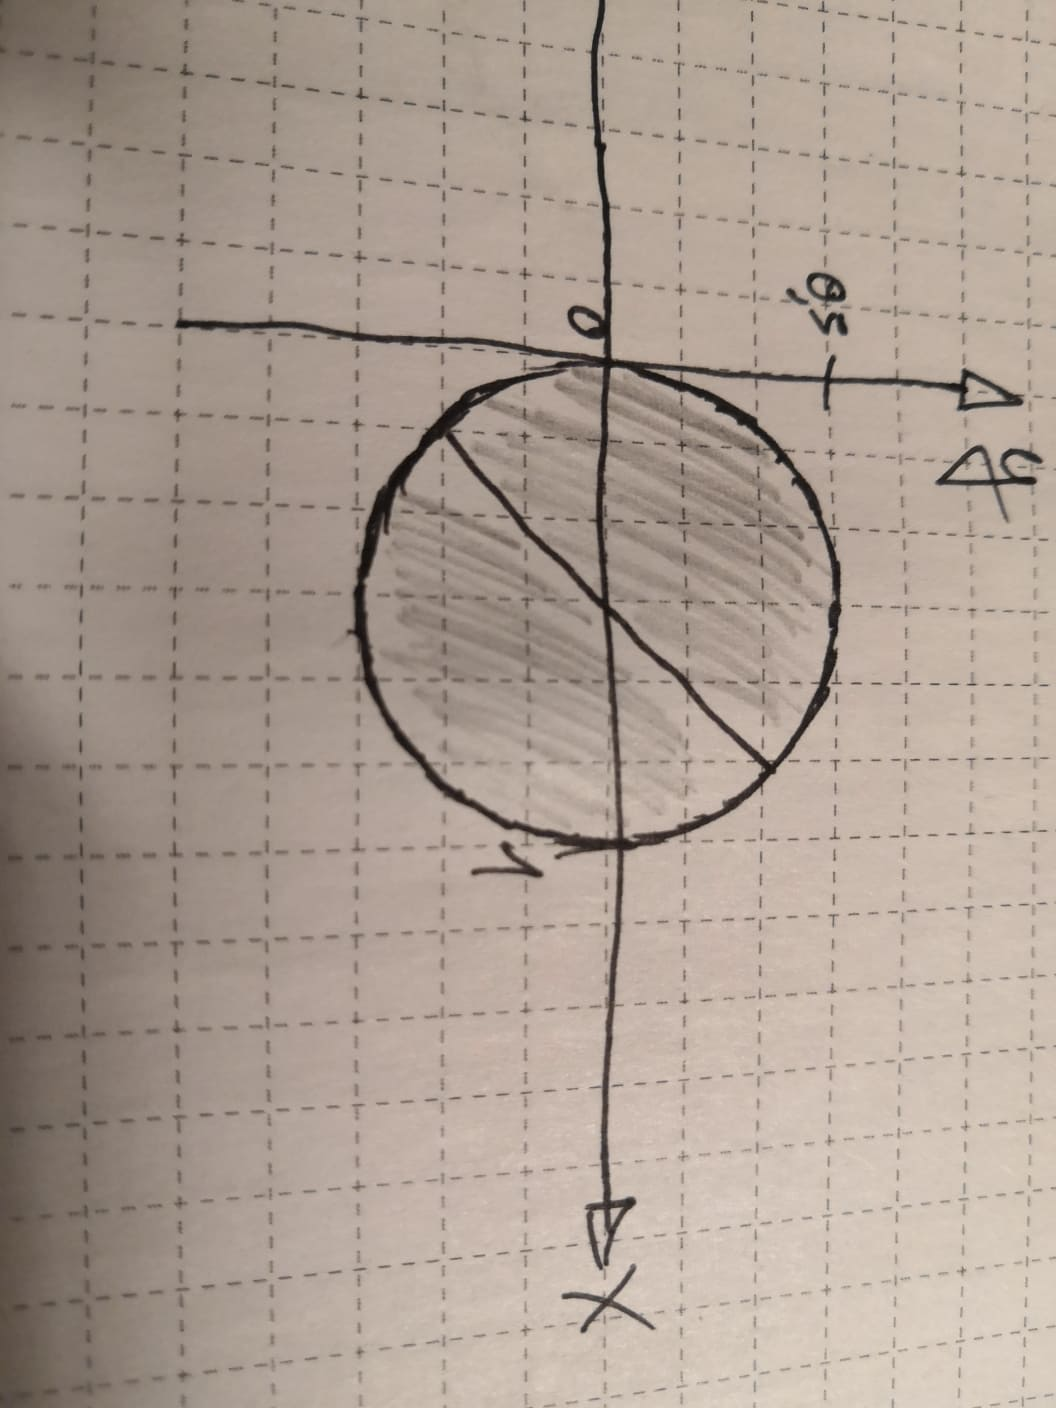
\includegraphics[scale=0.2,angle=90]{maaramispiirkond.jpg}}
\end{figure}\\
Kinnisuse kontrollimiseks vaatlen punkti $\left(\frac{1}{4},\frac{1}{4}\right)$. Kuna see sisaldub hulgas $\{(x,x)|x\in\mathbb{R}\}$, ei sisaldu see funktsiooni $f$ määramispiirkonnas. Leian selle punkti kauguse punktist $\left(\frac{1}{2},0\right)$:
\begin{equation*}
d\left(\left(\frac{1}{4},\frac{1}{4}\right),\left(\frac{1}{2},0\right)\right)=\sqrt{\left(\frac{1}{4}-\frac{1}{2}\right)^2+\left(\frac{1}{4}\right)^2}=\sqrt{\frac{2}{4^2}}=\frac{1}{2\sqrt{2}}<\frac{1}{2}
\end{equation*}
Seega see punkt sisaldub keras $\overline{B}\left(\left(\frac{1}{2},0\right),\frac{1}{2}\right)$. Hulk $\{(x,x)|x\in\mathbb{R}\}$ on joone jälg, seega kuna punkt $\left(\frac{1}{4},\frac{1}{4}\right)$ asub ümbritseva kera sees, on igas tema ümbruses punkte funktsiooni $f$ määramispiirkonnast kuid ta ise ei ole funktsiooni $f$ määramispiirkonnas, seega ta on määramispiirkonna rajapunkt ning kuna ta ei sisaldu määramispiirkonnas, ei ole määramispiirkond kinnine.\\
Määramispiirkond ei ole ka lahtine, kuna enamus kinnise kera $\overline{B}\left(\left(\frac{1}{2},0\right),\frac{1}{2}\right)$ rajapunktid asuvad määramispiirkonnas, kuid nad ei ole sisepunktid.\\
Seega ei ole funktsiooni $f$ määramispiirkond ei kinnine ega lahtine.\pagebreak\\
\textbf{2. }Lähtudes funktsiooni piirväärtuse definitsioonist, tõestada, et
\begin{equation*}
\lim_{x,y\to1,0}\frac{x+y^2}{y^4}=\infty
\end{equation*}
\textbf{Lahendus:}\\
Funktsiooni piirväärtuse definitsiooni kohaselt kehtib see piirväärtus parajasti siis, kui kehtib
\begin{equation*}
\forall N>0\ \exists\delta>0:[(x,y)\in\mathbb{R}^2,0<d((x,y),(1,0))<\delta]\Rightarrow\frac{x+y^2}{y^4}>N
\end{equation*}
$d((x,y),(1,0))<\delta$ saab ümber kirjutada kui $\sqrt{(x-1)^2+y^2}<\delta$ ehk $(x-1)^2+y^2<\delta^2$, millest saame, et $(x-1)^2<\delta^2\Leftrightarrow |x-1|<\delta\Rightarrow x-1<\delta$ ning $|y|<\delta\Rightarrow y<\delta$.\\
Funktsiooni $\frac{x+y^2}{y^4}$ saab ümber kirjutada kujule: $\frac{x+y^2}{y^4}=\frac{x}{y^4}+\frac{1}{y^2}>\frac{x}{\delta^4}+\frac{1}{\delta^2}$.\\
Lisan lisatingimuse, et $\delta\leq1$. Kuna kehtib $|x-1|<\delta$, saame $|x-1|<1\Leftrightarrow -1<x-1<1\Leftrightarrow 0<x<2$. Seega saame $\frac{x}{\delta^4}+\frac{1}{\delta^2}>\frac{0}{\delta^4}+\frac{1}{\delta^2}=\frac{1}{\delta^2}$\\
Seega kui valida $\delta=\min\{1,\frac{1}{\sqrt{\varepsilon}}\}$, saab väita et kui kehtib $d((x,y),(1,0))<\delta$, siis kehtib ka $\frac{x+y^2}{y^4}<\frac{1}{\delta^2}=\frac{1}{(\frac{1}{\sqrt{\varepsilon}})^2}=\varepsilon$, mida oligi tarvis tõestada.
\pagebreak\\
% Kiisu:       _
%             / )
%   /\___/\  ( (
%  /  0 0  \  \ \
%  \ ~(*)~ /   ) )
%   \  ^  /   / /
\textbf{3.} Teha kindlaks, kas funktsioon $f$ on pidev punktis $(0,0)$, kui
\begin{equation*}
f(x,y)=
\left\{
\begin{aligned}
&\frac{x^2y^3}{x^4+y^4}, && \text{kui } x^2+y^2\neq0;\\
&0, && \text{kui } x^2+y^2=0.
\end{aligned}
\right.
\end{equation*}
\textbf{Lahendus:}\\
Pidevuse definitsiooni järgi on funktsioon $f$ pidev punktis $(0,0)$ parajasti siis, kui kehtib $\lim_{x,y\to 0,0}f=f(0,0)$. Kontrollin selle tõesust.\\
$f(0,0)=0$ kuna $0^2+0^2=0$.\\
Viin piirväärtuse $\lim_{x,y\to 0,0}f=\lim_{x,y\to 0,0}\frac{x^2y^3}{x^4+y^4}$ polaarkoordinaatide süsteemi muutujavahetustega $x=r\cos \varphi$ ja $y=r\sin\varphi$:
\begin{gather*}
\begin{aligned}
\lim_{x,y\to 0,0}\frac{x^2y^3}{x^4+y^4}&=\lim_{r\to 0}\frac{r^2(\cos^2\varphi)\ r^3(\sin^3\varphi)}{r^4\cos^4\varphi+r^4\sin^4\varphi}\\
&=\lim_{r\to 0}\frac{r^5\cos^2\varphi\ \sin^3\varphi}{r^4(\cos^4\varphi+\sin^4\varphi)}\\
&=\lim_{r\to 0}r\frac{\cos^2\varphi\ \sin^3\varphi}{\cos^4\varphi+\sin^4\varphi}
\end{aligned}
\end{gather*}
Saadud murru nimetaja on tõkestatud ja selle väärtus ei ületa kindlasti 1, kuna siinus ja koosinus funktsioonid ei ületa 1. Murru lugeja on suurem kui null kuna see on summa kahest arvust, mis on paarisarvulises astmes, nii et kumbki et saa negatiivne olla ja siinus ja koosinusfunktsioon ei saa korraga 0 olla. Seega on terve murd tõkestatud ja tõkestatud arv korda nullile lähenev väärtus on 0, seega piirväärtus on null. Ehk kehtib $\lim_{x,y\to 0,0}f=\lim_{x,y\to 0,0}\frac{x^2y^3}{x^4+y^4}=0=f(0,0)$, mida oligi tarvis näidata.
\end{document}